%   ------------------------------------------------------------------------
\FloatBarrier
\section{Vidu}
\label{s.viduApendice}

\begin{figure}[htbp]
    \centering
    \caption{\small Processo da utilização do Vidu em junho/2025}
    \label{fig:vidu1}
    \begin{subfigure}{0.75\linewidth}
        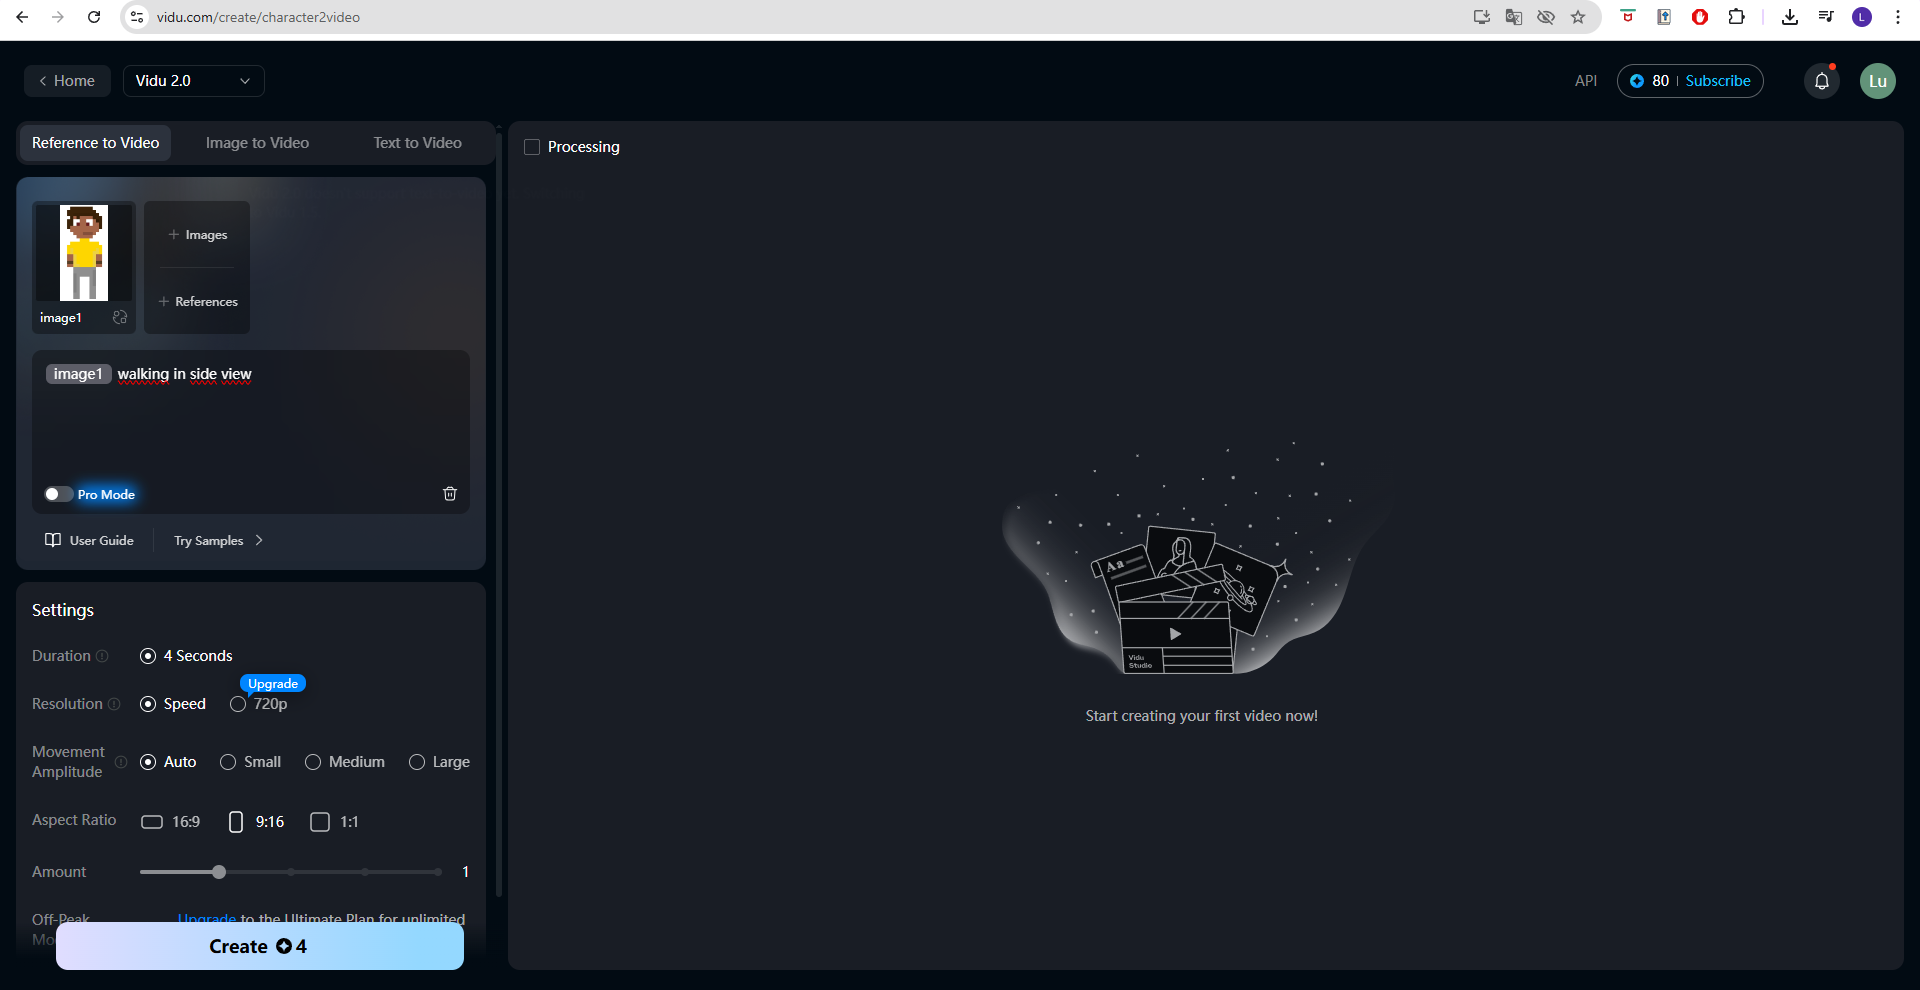
\includegraphics[width=1\linewidth]{figs/vidu/tela.PNG}
        \caption{\small Prompt}
        \label{fig:vidu1a}
    \end{subfigure}
    \begin{subfigure}{0.2\linewidth}
        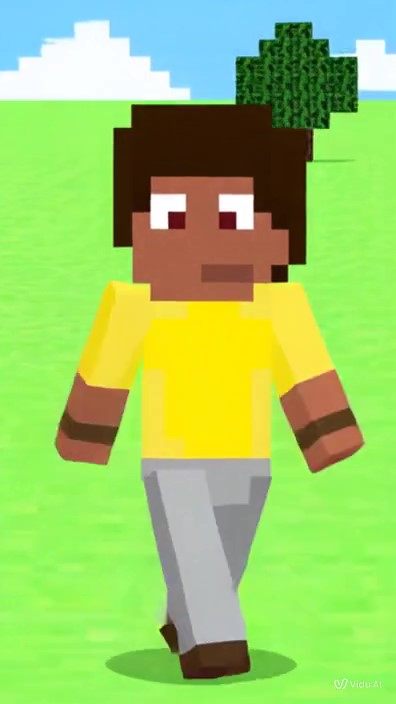
\includegraphics[width=1\linewidth]{figs/vidu/frame1.jpg}
        \caption{\small Frame do vídeo gerado}
        \label{fig:vidu1b}
    \end{subfigure}
    \begin{subfigure}{0.75\linewidth}
        \centering
        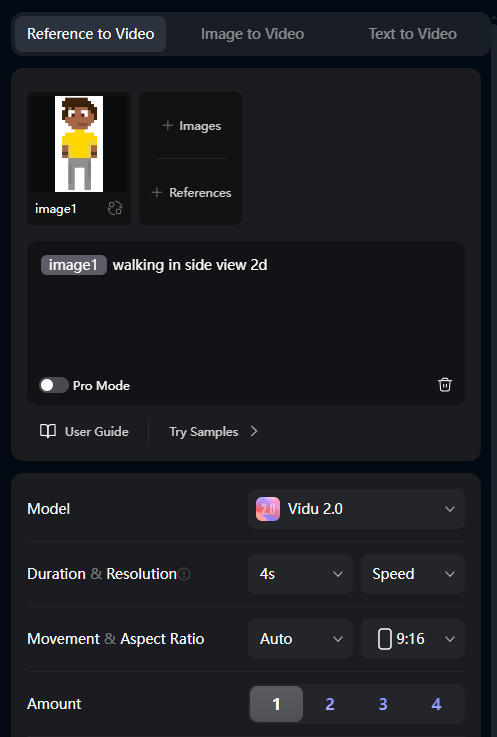
\includegraphics[width=0.4\linewidth]{figs/vidu/tela2_real.PNG}
        \caption{\small Prompt adicionando a palavra 2D}
        \label{fig:vidu1c}
    \end{subfigure}
    \begin{subfigure}{0.2\linewidth}
        
\includegraphics[width=1\linewidth]{figs/vidu/frame2.jpg}
        \caption{\small Frame do vídeo gerado}
        \label{fig:vidu1d}
    \end{subfigure}
    \begin{subfigure}{0.75\linewidth}
        \centering
        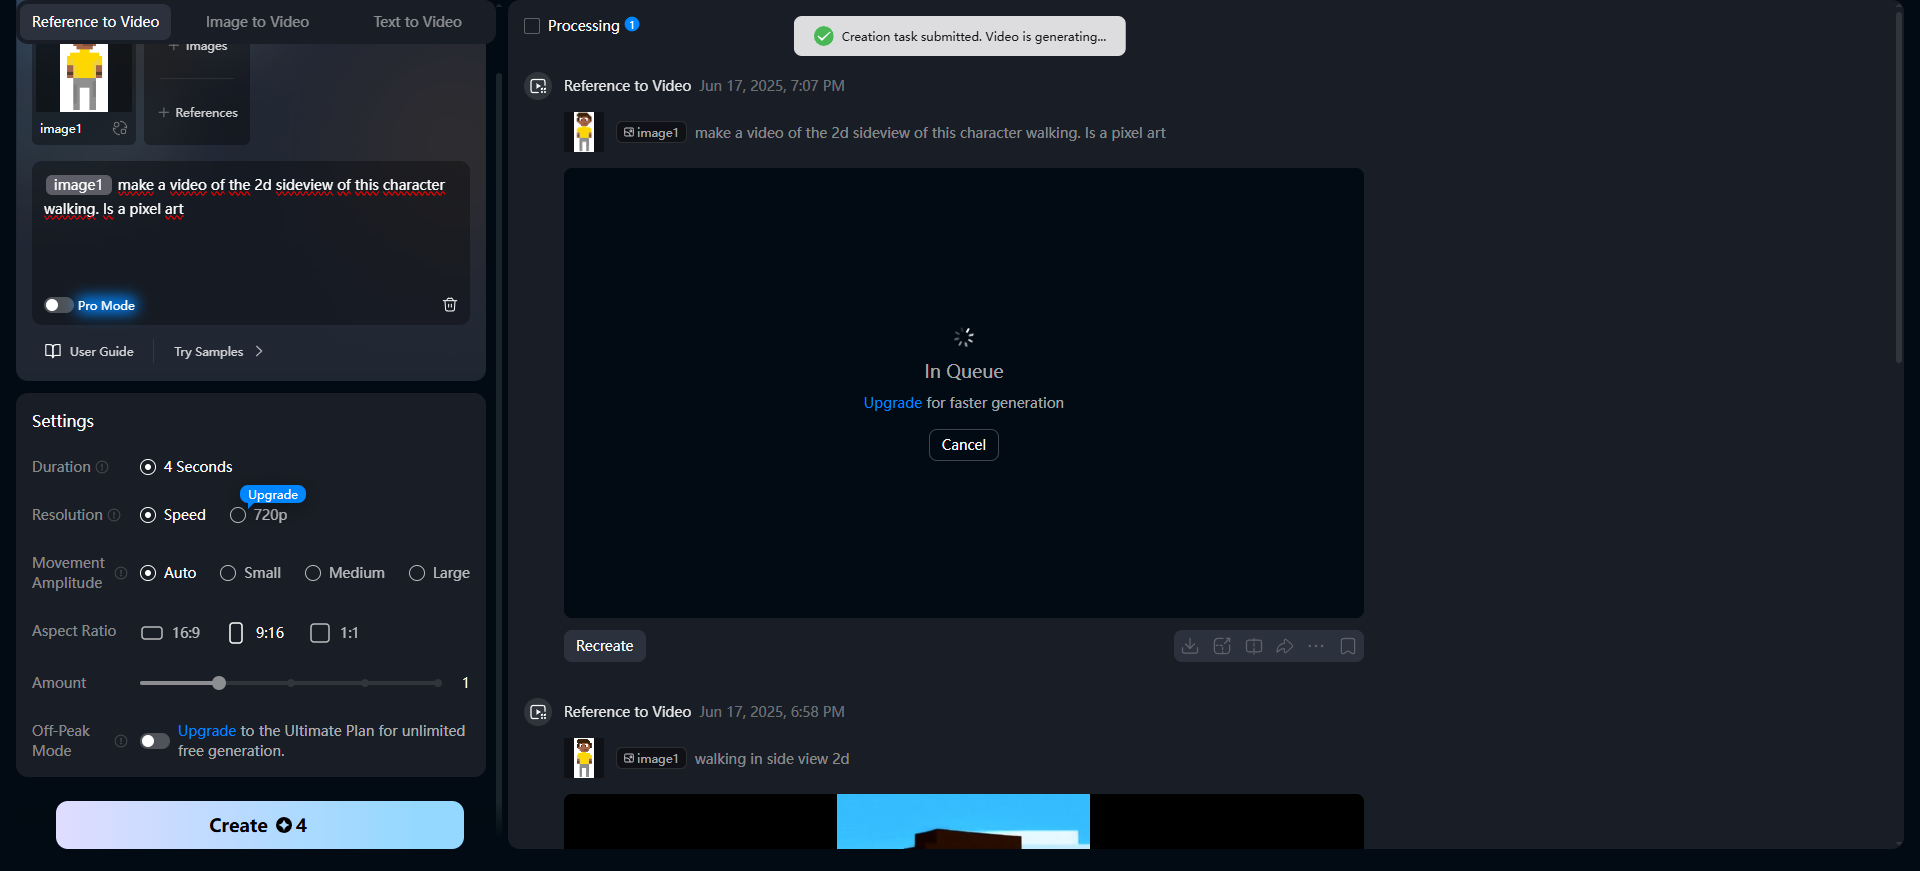
\includegraphics[width=1\linewidth]{figs/vidu/tela2.PNG}
        \caption{\small Prompt adicionando a palavra pixel art e não usando o imagem 1 como sujeito}
        \label{fig:vidu1e}
    \end{subfigure}
    \begin{subfigure}{0.2\linewidth}
        
\includegraphics[width=1\linewidth]{figs/vidu/frame3.jpg}
        \caption{\small Frame do vídeo gerado}
        \label{fig:vidu1f}
    \end{subfigure}
    \legend{\small Fonte: Elaborada pela autora, utilizando a ferramenta Vidu.}
\end{figure}

\begin{figure}[htbp]
    \centering
    \caption{\small Processo da utilização 1 do Vidu em julho/2025}
    \label{fig:vidu2}
    \begin{subfigure}{0.4\linewidth}
        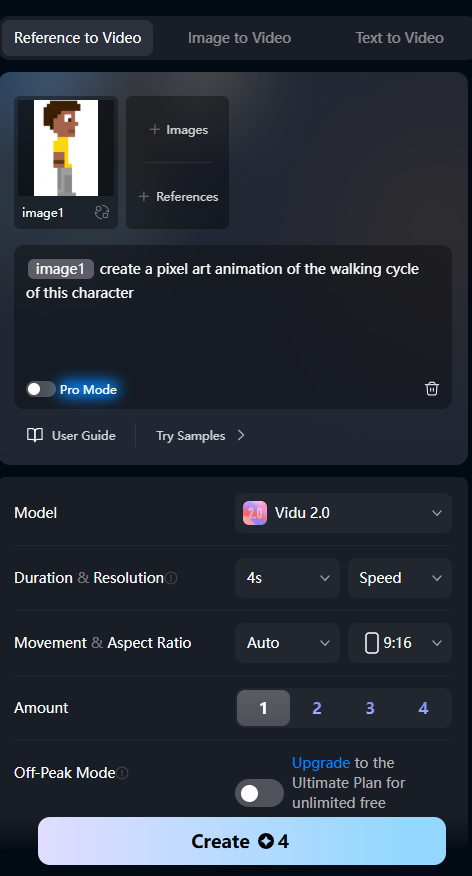
\includegraphics[width=1\linewidth]{figs/vidu/tela3.PNG}
        \caption{\small Prompt}
        \label{fig:vidu2a}
    \end{subfigure}
    \begin{subfigure}{0.2\linewidth}
        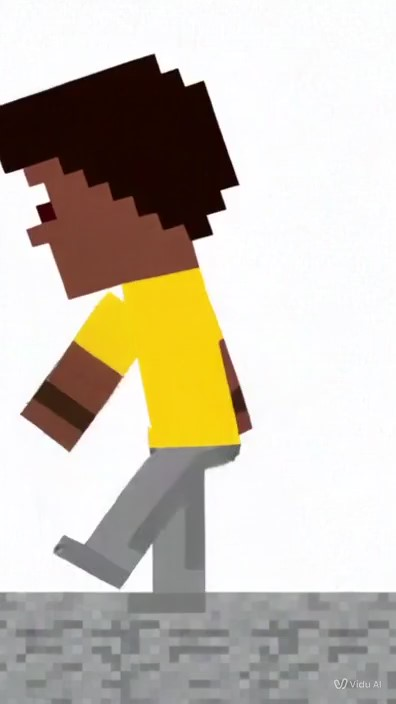
\includegraphics[width=1\linewidth]{figs/vidu/frame4.jpg}
        \caption{\small Frame do vídeo 1 gerado}
        \label{fig:vidu2b}
    \end{subfigure}
    \begin{subfigure}{0.2
    \linewidth}
        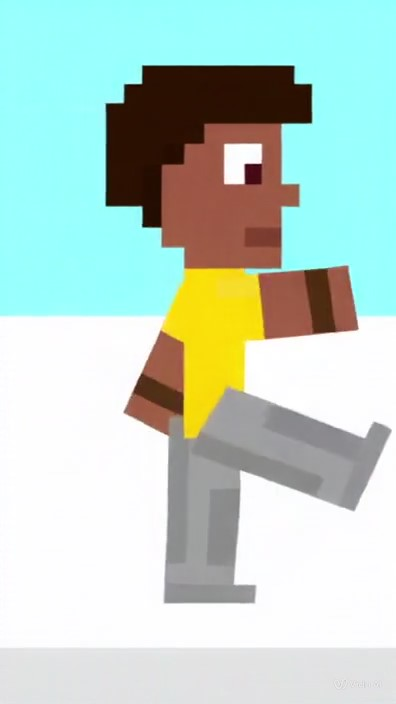
\includegraphics[width=1\linewidth]{figs/vidu/frame4.2.jpg}
        \caption{\small Frame do vídeo 2 gerado}
        \label{fig:vidu2c}
    \end{subfigure}

    \legend{\small Fonte: Elaborada pela autora, utilizando a ferramenta Vidu.}
\end{figure}

\begin{figure}[htbp]
    \centering
    \caption{\small Processo da utilização 2 do Vidu em julho/2025}
    \label{fig:vidu3}
    \begin{subfigure}{0.4\linewidth}
        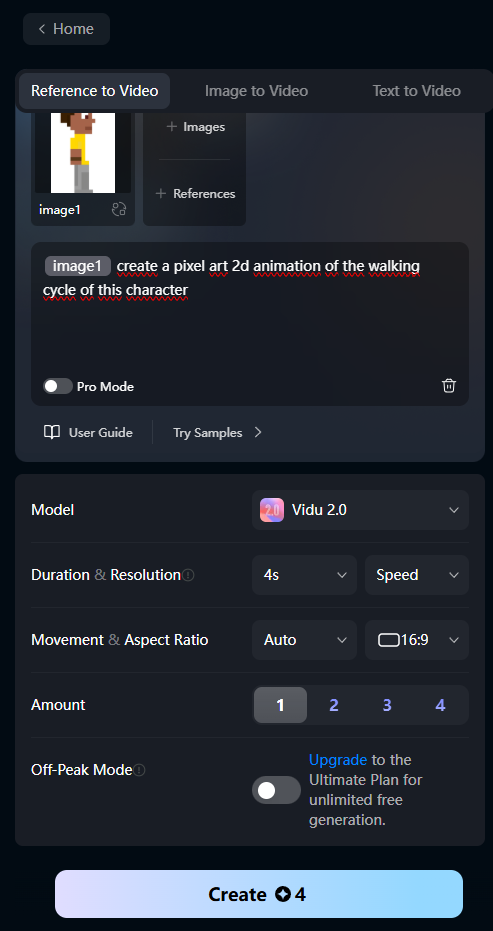
\includegraphics[width=1\linewidth]{figs/vidu/tela4.PNG}
        \caption{\small Prompt adicionando a palavra 2D e mudança de proporção}
        \label{fig:vidu3a}
    \end{subfigure}
    \begin{subfigure}{0.4\linewidth}
        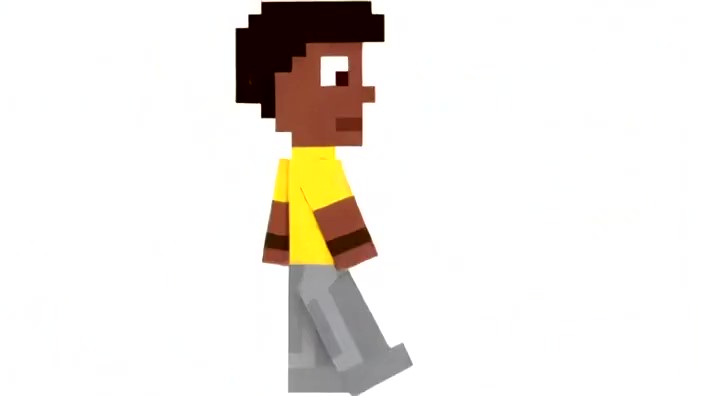
\includegraphics[width=1\linewidth]{figs/vidu/frame5_2D.jpg}
        \caption{\small Frame 1 do vídeo gerado, aparentando ser 2D}
        \label{fig:vidu3b}
    \end{subfigure}
    \begin{subfigure}{0.4\linewidth}
        
\includegraphics[width=1\linewidth]{figs/vidu/frame5_3D.jpg}
        \caption{\small Frame 2 do vídeo gerado, em 3D}
        \label{fig:vidu3c}
    \end{subfigure}

    \legend{\small Fonte: Elaborada pela autora, utilizando a ferramenta Vidu.}
\end{figure}

\begin{figure}[htbp]
    \centering
    \caption{\small Processo da utilização 3 do Vidu em julho/2025}
    \label{fig:vidu4}
    \begin{subfigure}{0.6\linewidth}
        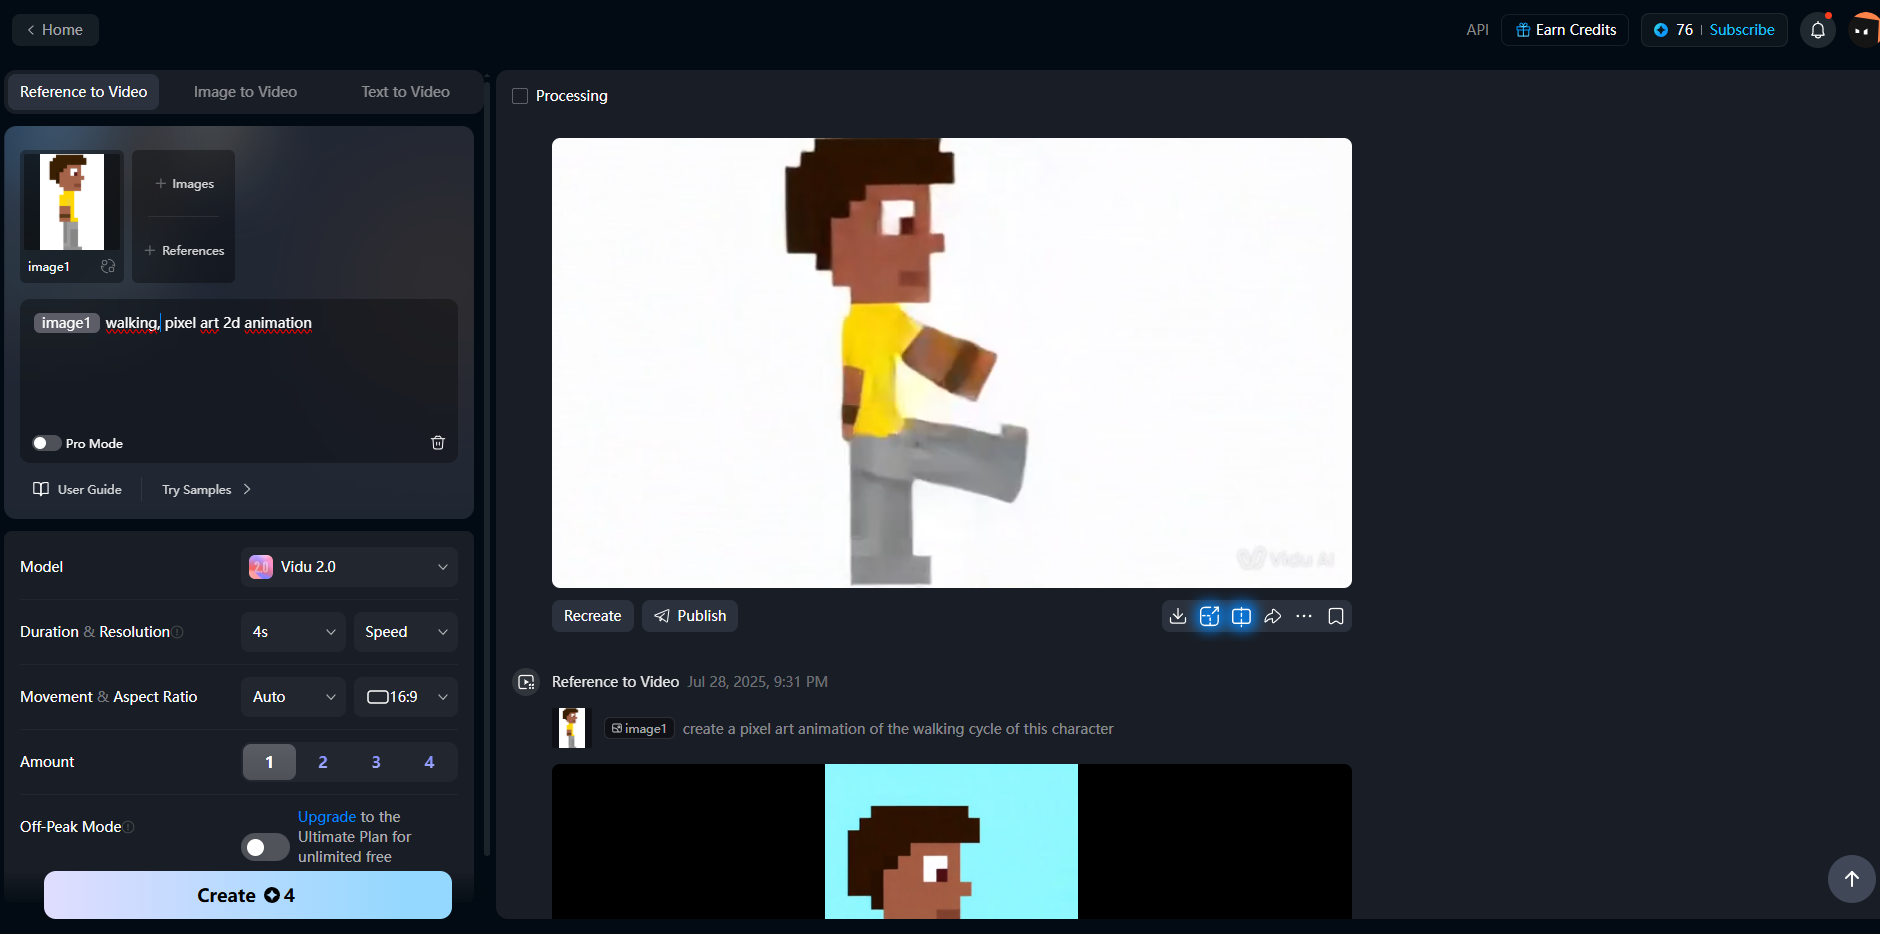
\includegraphics[width=1\linewidth]{figs/vidu/tela5.PNG}
        \caption{\small Prompt utilizando a tag da imagem como sujeito}
        \label{fig:vidu4a}
    \end{subfigure}
    \begin{subfigure}{0.35\linewidth}
        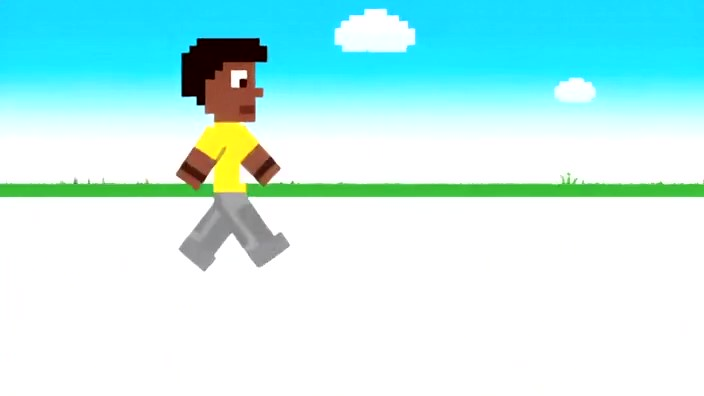
\includegraphics[width=1\linewidth]{figs/vidu/frame6.jpg}
        \caption{\small Frame do vídeo gerado}
        \label{fig:vidu4b}
    \end{subfigure}
    \legend{\small Fonte: Elaborada pela autora, utilizando a ferramenta Vidu.}
\end{figure}

\begin{figure}[htbp]
    \centering
    \caption{\small Processo da utilização 4 do Vidu em julho/2025}
    \label{fig:vidu5}
    \begin{subfigure}{0.4\linewidth}
        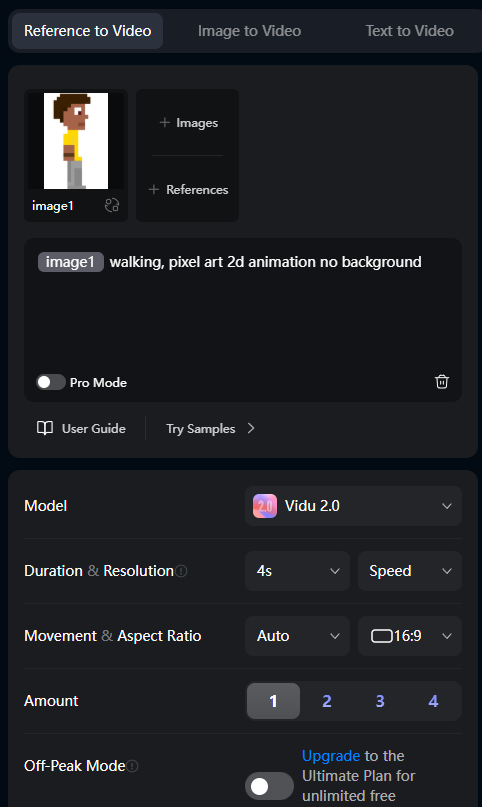
\includegraphics[width=1\linewidth]{figs/vidu/tela5_2.PNG}
        \caption{\small Prompt especificando o fundo sem nada}
        \label{fig:vidu5a}
    \end{subfigure}
    \begin{subfigure}{0.4\linewidth}
        
\includegraphics[width=1\linewidth]{figs/vidu/frame6_2.jpg}
        \caption{\small Frame do vídeo gerado}
        \label{fig:vidu5b}
    \end{subfigure}
    \legend{\small Fonte: Elaborada pela autora, utilizando a ferramenta Vidu.}
\end{figure}



\begin{figure}[htbp]
    \centering
    \caption{\small Tela da criação da referência da beliche no Vidu}
    \label{fig:viduReferenciaCama}
    \begin{subfigure}{0.4\linewidth}
        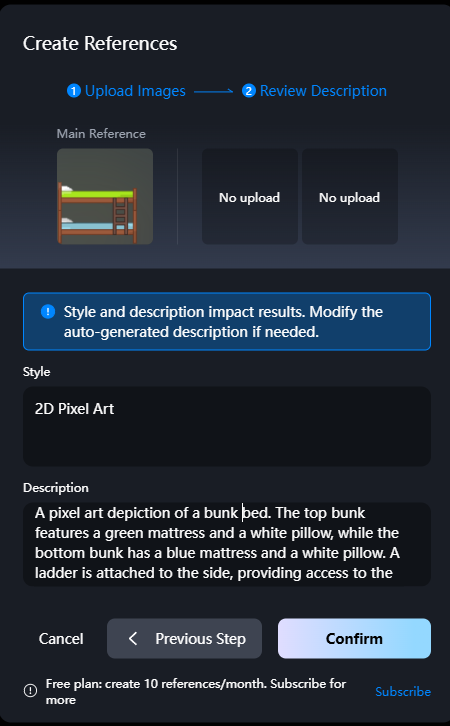
\includegraphics[width=1\linewidth]{figs/vidu/tela_referencia_beliche.PNG}
        \caption{\small Parte 1 da descrição}
        \label{fig:viduReferenciaCama1}
    \end{subfigure}
    \begin{subfigure}{0.45\linewidth}
        
\includegraphics[width=1\linewidth]{figs/vidu/tela_referencia_beliche2.PNG}
        \caption{\small Parte 2 da descrição}
        \label{fig:viduReferenciaCama2}
    \end{subfigure}
    \legend{\small Fonte: Elaborada pela autora.}
\end{figure}


\begin{figure}[htbp]
    \centering
    \caption{\small Tela da criação da referência da porta marrom no Vidu}
    \label{fig:viduReferenciaPortaA}
    \begin{subfigure}{0.4\linewidth}
        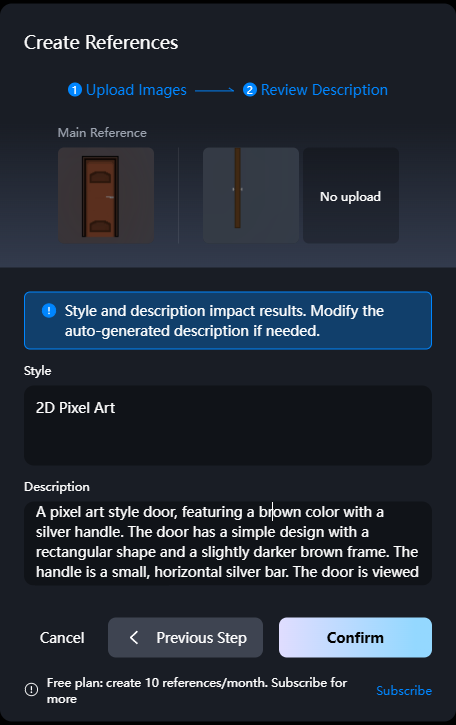
\includegraphics[width=1\linewidth]{figs/vidu/tela_referencia_porta.PNG}
        \caption{\small Parte 1 da descrição}
        \label{fig:viduReferenciaPortaA1}
    \end{subfigure}
    \begin{subfigure}{0.4\linewidth}
        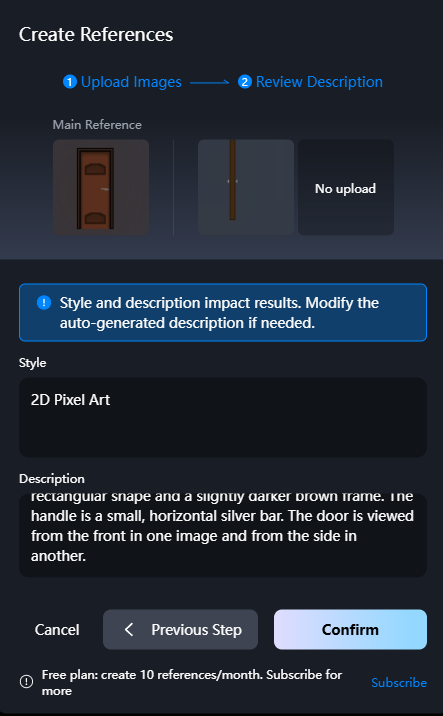
\includegraphics[width=1\linewidth]{figs/vidu/tela_referencia_porta_2.PNG}
        \caption{\small Parte 2 da descrição}
        \label{fig:viduReferenciaPortaA2}
    \end{subfigure}
    \legend{\small Fonte: Elaborada pela autora.}
\end{figure}

\begin{figure}[htbp]
    \centering
    \caption{\small Tela da criação da referência da porta cinza no Vidu}
    \label{fig:viduReferenciaPortaC}
    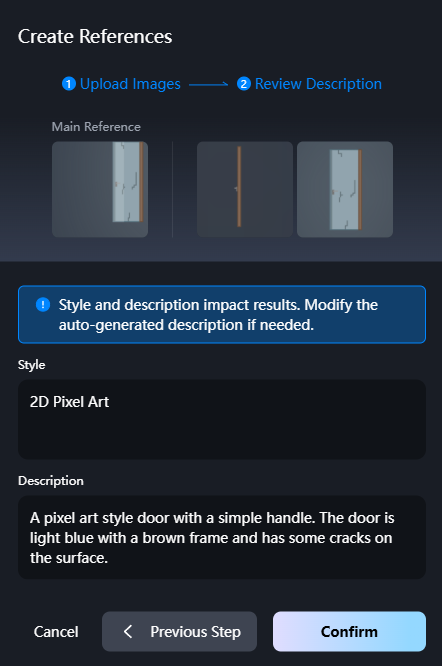
\includegraphics[width=0.4\linewidth]{figs/vidu/tela_referencia_porta_tutorial.PNG}
    \legend{\small Fonte: Elaborada pela autora.}
\end{figure}

\begin{figure}[htbp]
    \centering
    \caption{\small Tela da criação da referência do quarto do Pablo no Vidu}
    \label{fig:viduReferenciaQuarto}
    \begin{subfigure}{0.4\linewidth}
        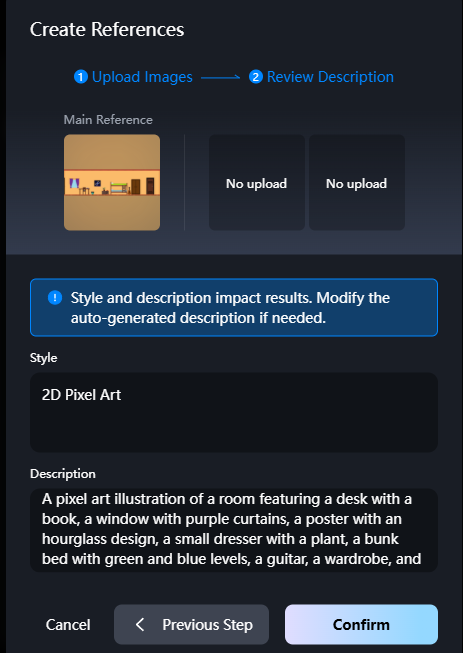
\includegraphics[width=1\linewidth]{figs/vidu/tela_referencia_quarto.PNG}
        \caption{\small Parte 1 da descrição}
        \label{fig:viduReferenciaQuarto1}
    \end{subfigure}
    \begin{subfigure}{0.4\linewidth}
        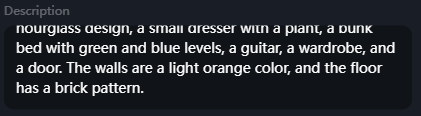
\includegraphics[width=1\linewidth]{figs/vidu/tela_referencia_quarto2.PNG}
        \caption{\small Parte 2 da descrição}
        \label{fig:viduReferenciaQuarto2}
    \end{subfigure}
    \legend{\small Fonte: Elaborada pela autora.}
\end{figure}

\begin{figure}[htbp]
    \centering
    \caption{\small Tela da criação da referência da cena do tutorial no Vidu}
    \label{fig:viduReferenciaTutorial}
    \begin{subfigure}{0.4\linewidth}
        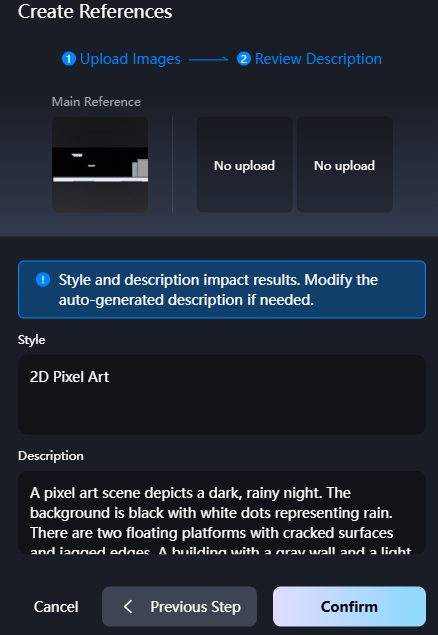
\includegraphics[width=1\linewidth]{figs/vidu/tela_referencia_tutorial.PNG}
        \caption{\small Parte 1 da descrição}
        \label{fig:viduReferenciaTutorial1}
    \end{subfigure}
    \begin{subfigure}{0.4\linewidth}
        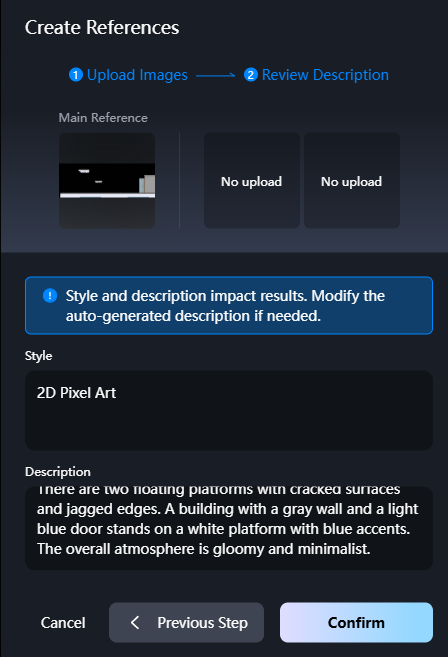
\includegraphics[width=1\linewidth]{figs/vidu/tela_referencia_tutorial_2.PNG}
        \caption{\small Parte 2 da descrição}
        \label{fig:viduReferenciaTutorial2}
    \end{subfigure}
    \legend{\small Fonte: Elaborada pela autora.}
\end{figure}


\begin{figure}[htbp]
    \centering
    \caption{\small Processo da utilização 1 do Vidu em agosto/2025}
    \label{fig:vidu6}
    \begin{subfigure}{0.35\linewidth}
        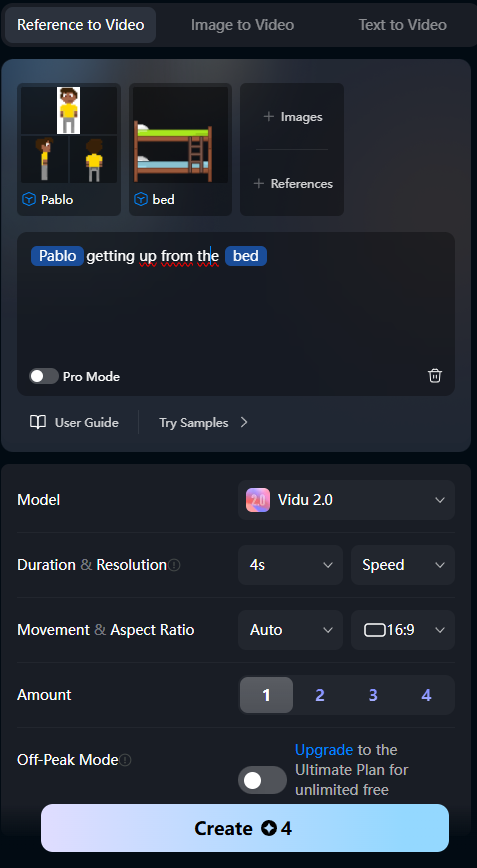
\includegraphics[width=1\linewidth]{figs/vidu/tela6.PNG}
        \caption{\small Prompt}
        \label{fig:vidu6a}
    \end{subfigure}
    \begin{subfigure}{0.55\linewidth}
        
\includegraphics[width=1\linewidth]{figs/vidu/frame6_real.jpg}
        \caption{\small Frame do vídeo gerado}
        \label{fig:vidu6b}
    \end{subfigure}
    \legend{\small Fonte: Elaborada pela autora, utilizando a ferramenta Vidu.}
\end{figure}

\begin{figure}[htbp]
    \centering
    \caption{\small Processo da utilização 2 do Vidu em agosto/2025}
    \label{fig:vidu7}
    \begin{subfigure}{0.35\linewidth}
        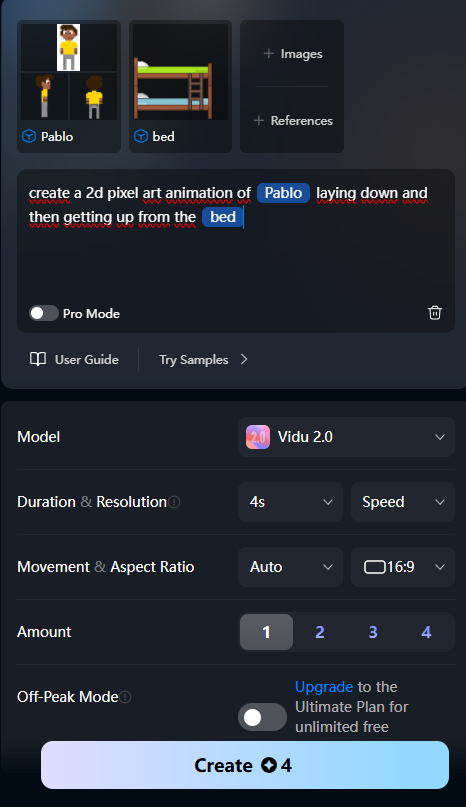
\includegraphics[width=1\linewidth]{figs/vidu/tela7.PNG}
        \caption{\small Prompt}
        \label{fig:vidu7a}
    \end{subfigure}
    \begin{subfigure}{0.55\linewidth}
        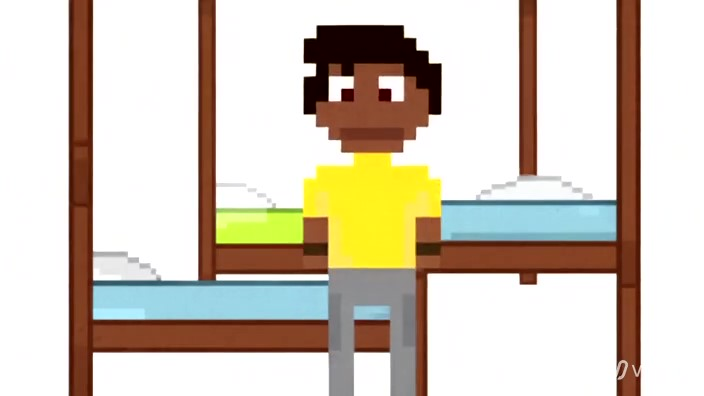
\includegraphics[width=1\linewidth]{figs/vidu/frame7.jpg}
        \caption{\small Frame do vídeo gerado}
        \label{fig:vidu7b}
    \end{subfigure}
    \legend{\small Fonte: Elaborada pela autora, utilizando a ferramenta Vidu.}
\end{figure}

\begin{figure}[htbp]
    \centering
    \caption{\small Processo da utilização 3 do Vidu em agosto/2025}
    \label{fig:vidu8}
    \begin{subfigure}{0.35\linewidth}
        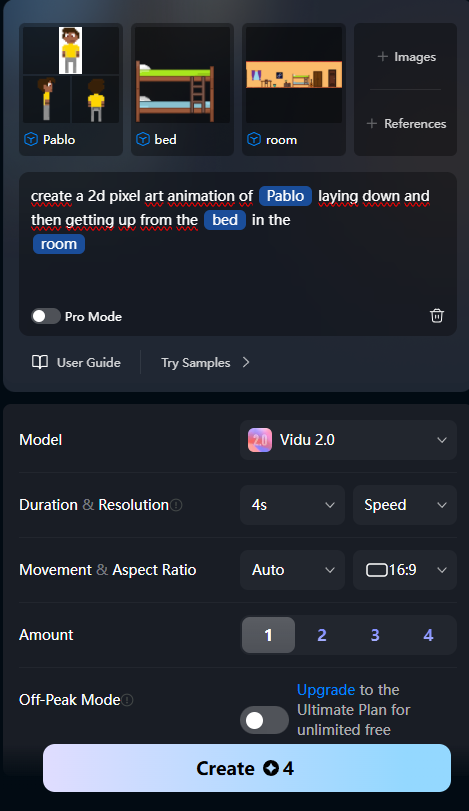
\includegraphics[width=1\linewidth]{figs/vidu/tela8.PNG}
        \caption{\small Prompt}
        \label{fig:vidu8a}
    \end{subfigure}
    \begin{subfigure}{0.55\linewidth}
        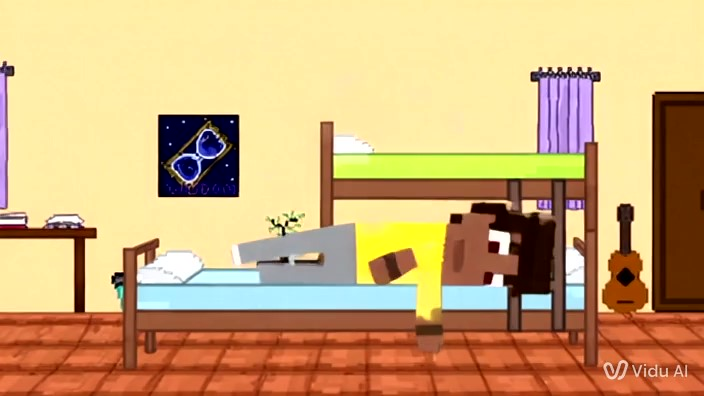
\includegraphics[width=1\linewidth]{figs/vidu/frame8.jpg}
        \caption{\small Frame do vídeo gerado}
        \label{fig:vidu8b}
    \end{subfigure}
    \legend{\small Fonte: Elaborada pela autora, utilizando a ferramenta Vidu.}
\end{figure}

\begin{figure}[htbp]
    \centering
    \caption{\small Processo da utilização 4 do Vidu em agosto/2025}
    \label{fig:vidu9}
    \begin{subfigure}{0.35\linewidth}
        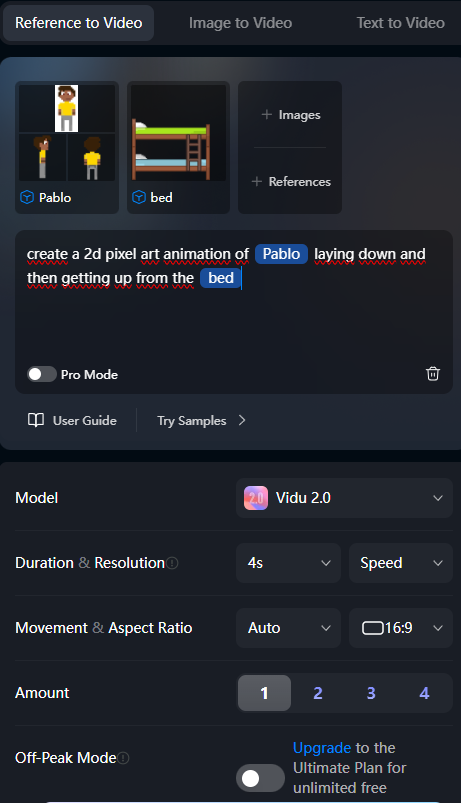
\includegraphics[width=1\linewidth]{figs/vidu/tela9.PNG}
        \caption{\small Prompt}
        \label{fig:vidu9a}
    \end{subfigure}
    \begin{subfigure}{0.55\linewidth}
        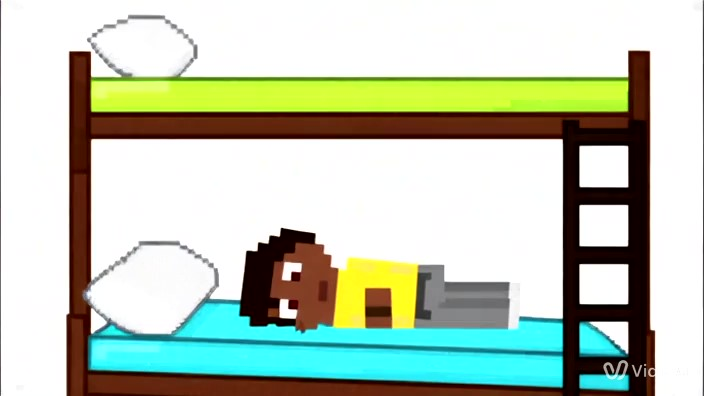
\includegraphics[width=1\linewidth]{figs/vidu/frame9.jpg}
        \caption{\small Frame do vídeo gerado}
        \label{fig:vidu9b}
    \end{subfigure}
    \legend{\small Fonte: Elaborada pela autora, utilizando a ferramenta Vidu.}
\end{figure}

\begin{figure}[htbp]
    \centering
    \caption{\small Edição da referência do personagem no Vidu}
    \label{fig:viduReferenciaPabloEditado}
    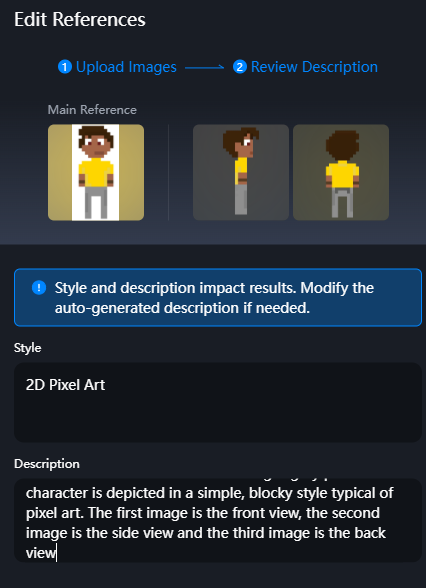
\includegraphics[width=0.4\linewidth]{figs/vidu/tela_referencia_2_editado2.PNG}
    \legend{\small Fonte: Elaborada pela autora.}
\end{figure}

\begin{figure}[htbp]
    \centering
    \caption{\small Processo da utilização 5 do Vidu em agosto/2025}
    \label{fig:vidu10}
    \begin{subfigure}{0.35\linewidth}
        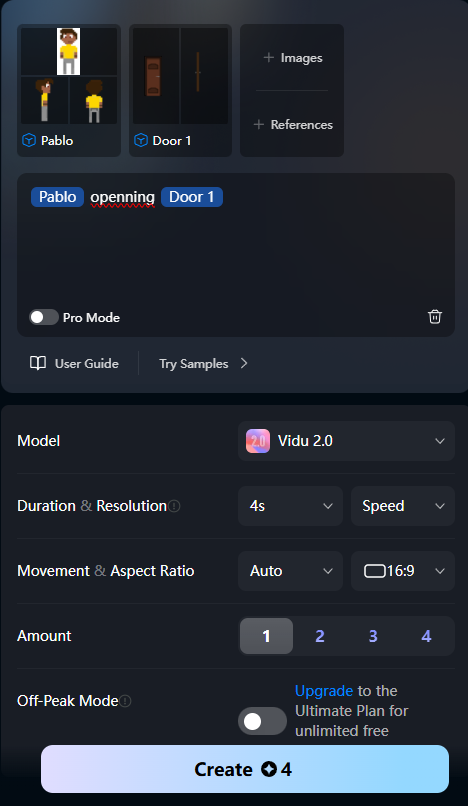
\includegraphics[width=1\linewidth]{figs/vidu/tela10.PNG}
        \caption{\small Prompt}
        \label{fig:vidu10a}
    \end{subfigure}
    \begin{subfigure}{0.55\linewidth}
        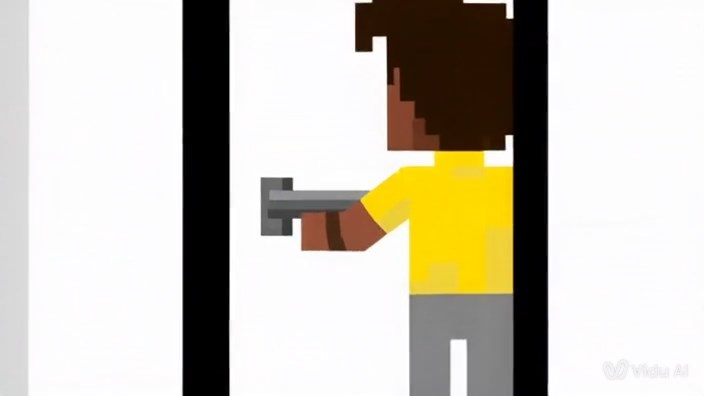
\includegraphics[width=1\linewidth]{figs/vidu/frame10.jpg}
        \caption{\small Frame do vídeo gerado}
        \label{fig:vidu10b}
    \end{subfigure}
    \legend{\small Fonte: Elaborada pela autora, utilizando a ferramenta Vidu.}
\end{figure}

\begin{figure}[htbp]
    \centering
    \caption{\small Processo da utilização 6 do Vidu em agosto/2025}
    \label{fig:vidu11}
    \begin{subfigure}{0.35\linewidth}
        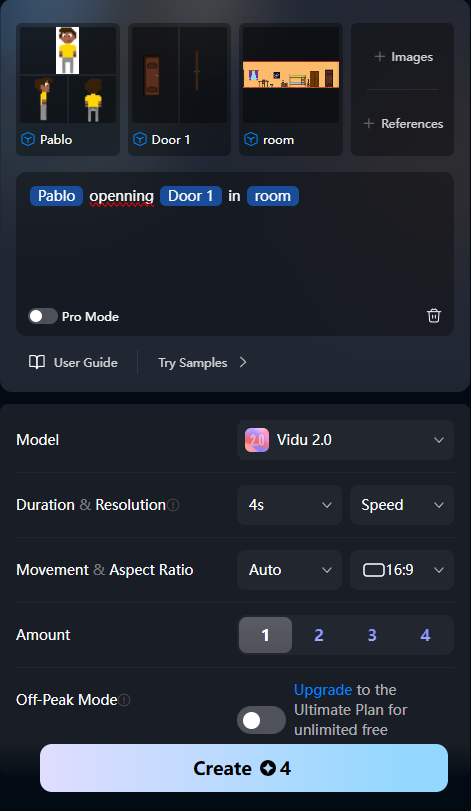
\includegraphics[width=1\linewidth]{figs/vidu/tela11.PNG}
        \caption{\small Prompt}
        \label{fig:vidu11a}
    \end{subfigure}
    \begin{subfigure}{0.55\linewidth}
        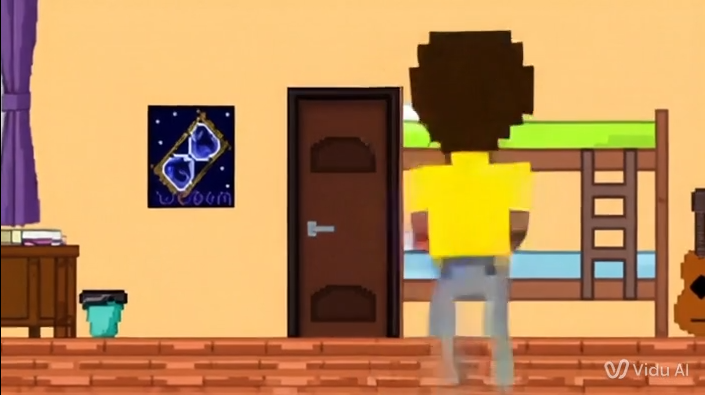
\includegraphics[width=1\linewidth]{figs/vidu/frame11.PNG}
        \caption{\small Frame do vídeo gerado}
        \label{fig:vidu11b}
    \end{subfigure}
    \legend{\small Fonte: Elaborada pela autora, utilizando a ferramenta Vidu.}
\end{figure}

\begin{figure}[htbp]
    \centering
    \caption{\small Processo da utilização 7 do Vidu em agosto/2025}
    \label{fig:vidu12}
    \begin{subfigure}{0.35\linewidth}
        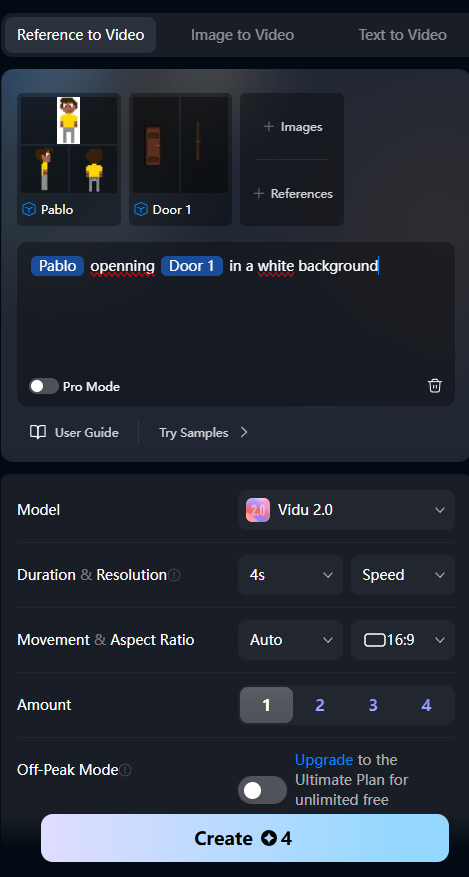
\includegraphics[width=1\linewidth]{figs/vidu/tela12.PNG}
        \caption{\small Prompt}
        \label{fig:vidu12a}
    \end{subfigure}
    \begin{subfigure}{0.55\linewidth}
        
\includegraphics[width=1\linewidth]{figs/vidu/frame12.jpg}
        \caption{\small Frame do vídeo gerado}
        \label{fig:vidu12b}
    \end{subfigure}
    \legend{\small Fonte: Elaborada pela autora, utilizando a ferramenta Vidu.}
\end{figure}

\begin{figure}[htbp]
    \centering
    \caption{\small Processo da utilização 8 do Vidu em agosto/2025}
    \label{fig:vidu13}
    \begin{subfigure}{0.42\linewidth}
        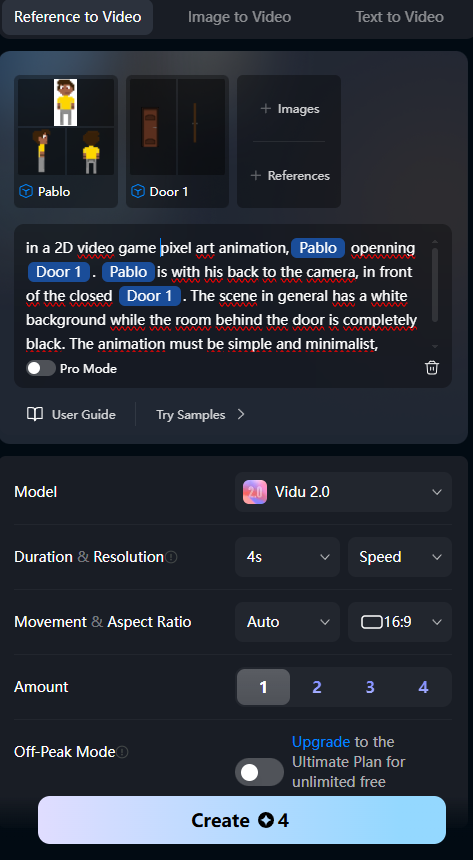
\includegraphics[width=1\linewidth]{figs/vidu/tela13.PNG}
        \caption{\small Prompt}
        \label{fig:vidu13a}
    \end{subfigure}
    \begin{subfigure}{0.52\linewidth}
        
\includegraphics[width=1\linewidth]{figs/vidu/tela13_resto.PNG}
        \caption{\small Continuação do prompt}
        \label{fig:vidu13b}
    \end{subfigure}
    \begin{subfigure}{0.55\linewidth}
        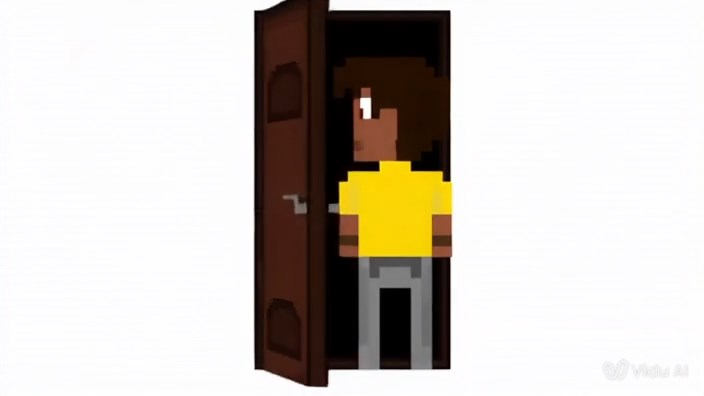
\includegraphics[width=1\linewidth]{figs/vidu/frame13.jpg}
        \caption{\small Frame do vídeo gerado}
        \label{fig:vidu13c}
    \end{subfigure}
    \legend{\small Fonte: Elaborada pela autora, utilizando a ferramenta Vidu.}
\end{figure}


\begin{figure}[htbp]
    \centering
    \caption{\small Processo de geração da animação de pulo pela funcionalidade Referência para vídeo no Vidu}
    \label{fig:viduPulo1}
    \begin{subfigure}{0.55\linewidth}
        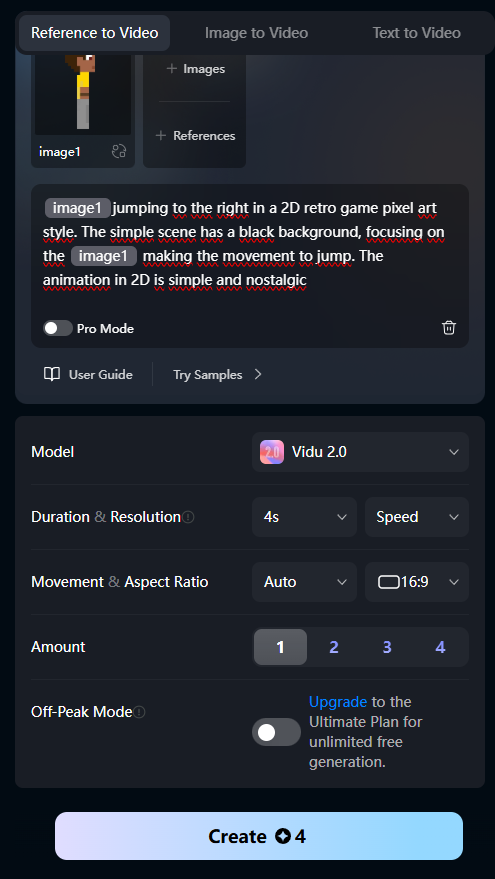
\includegraphics[width=1\linewidth]{figs/vidu/PULO_tela01.PNG}
        \caption{\small Prompt}
        \label{fig:viduPulo1a}
    \end{subfigure}
    \begin{subfigure}{0.45\linewidth}
        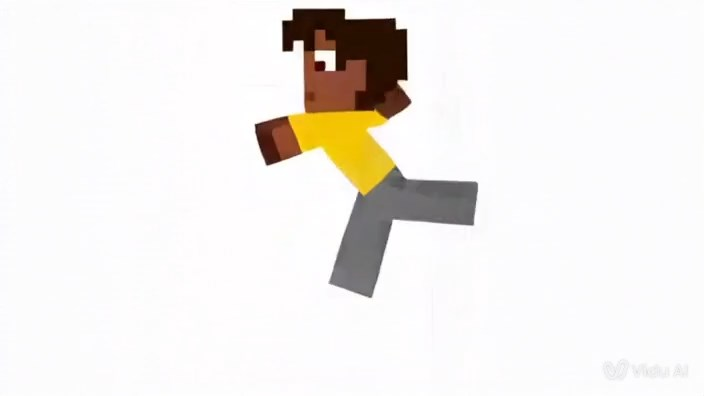
\includegraphics[width=1\linewidth]{figs/vidu/framePulo1.jpg}
        \caption{\small Frame do vídeo 1 gerado}
        \label{fig:viduPulo1b}
    \end{subfigure}
    \begin{subfigure}{0.45\linewidth}
        
\includegraphics[width=1\linewidth]{figs/vidu/framePulo1_2.jpg}
        \caption{\small Frame do vídeo gerado}
        \label{fig:viduPulo1c}
    \end{subfigure}
    \legend{\small Fonte: Elaborada pela autora, utilizando a ferramenta Vidu.}
\end{figure}

\begin{figure}[htbp]
    \centering
    \caption{\small Processo de geração da animação 1 da porta no Vidu }
    \label{fig:viduPorta1}
    \begin{subfigure}{0.42\linewidth}
        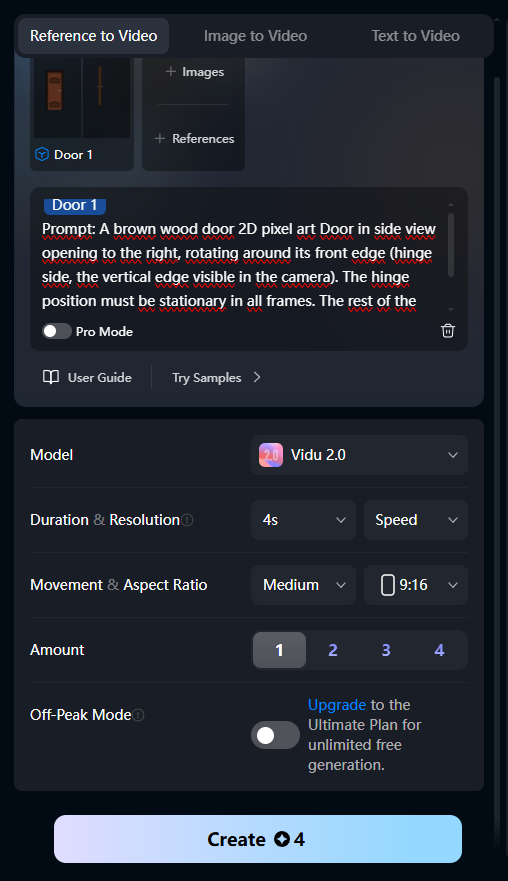
\includegraphics[width=1\linewidth]{figs/vidu/porta_tela1.PNG}
        \caption{\small Prompt}
        \label{fig:viduPorta1a}
    \end{subfigure}
    \begin{subfigure}{0.42\linewidth}
        
\includegraphics[width=1\linewidth]{figs/vidu/porta_tela2.PNG}
        \caption{\small Prompt}
        \label{fig:viduPorta1b}
    \end{subfigure}
    \begin{subfigure}{0.32\linewidth}
        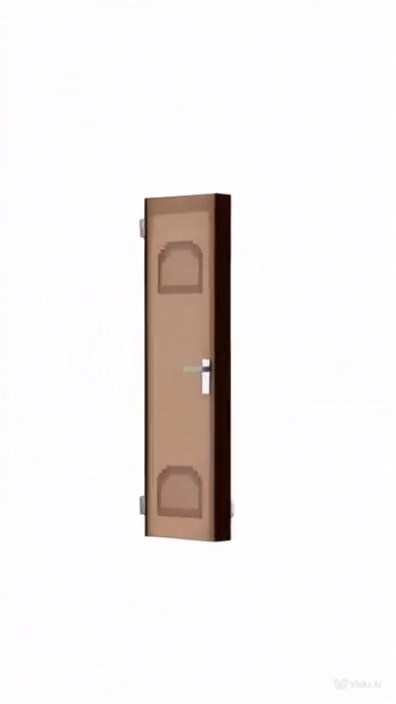
\includegraphics[width=1\linewidth]{figs/vidu/framePorta1.jpg}
        \caption{\small Continuação do prompt}
        \label{fig:viduPorta1c}
    \end{subfigure}
    \legend{\small Fonte: Elaborada pela autora, utilizando a ferramenta Vidu.}
\end{figure}

\begin{figure}[htbp]
    \centering
    \caption{\small Processo de geração da animação 2 da porta no Vidu }
    \label{fig:viduPorta2}
    \begin{subfigure}{0.42\linewidth}
        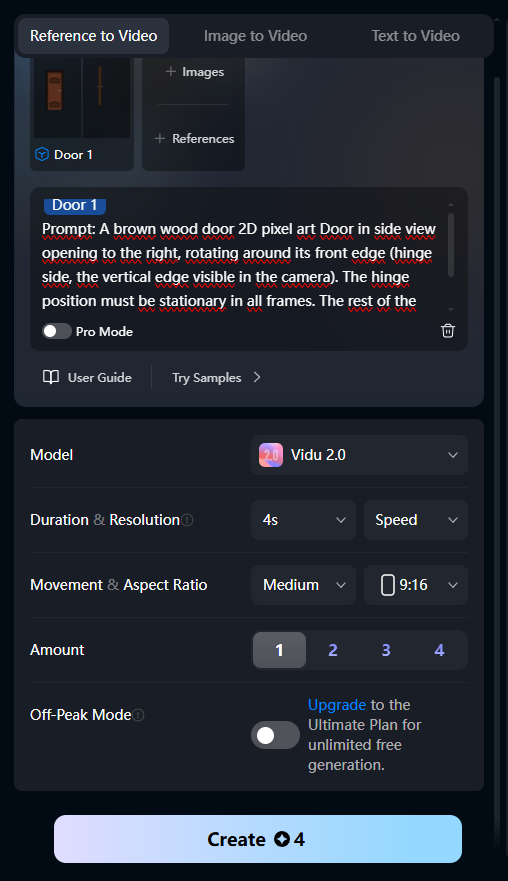
\includegraphics[width=1\linewidth]{figs/vidu/porta_tela1.PNG}
        \caption{\small Prompt}
        \label{fig:viduPorta2a}
    \end{subfigure}
    \begin{subfigure}{0.42\linewidth}
        \includegraphics[width=1\linewidth]{figs/vidu/porta_tela3.PNG}
        \caption{\small Prompt}
        \label{fig:viduPorta2b}
    \end{subfigure}
    \begin{subfigure}{0.32\linewidth}
        \includegraphics[width=1\linewidth]{figs/vidu/framePorta2.jpg}
        \caption{\small Continuação do prompt}
        \label{fig:viduPorta2c}
    \end{subfigure}
    \legend{\small Fonte: Elaborada pela autora, utilizando a ferramenta Vidu.}
\end{figure}

\begin{figure}[htbp]
    \centering
    \caption{\small Animação da porta cinza pela funcionalidade Imagem para vídeo no Vidu }
    \label{fig:vidu14}
    \begin{subfigure}{0.42\linewidth}
        \includegraphics[width=1\linewidth]{figs/vidu/tela14.PNG}
        \caption{\small Prompt}
        \label{fig:vidu14a}
    \end{subfigure}
    \begin{subfigure}{0.42\linewidth}
        \includegraphics[width=1\linewidth]{figs/vidu/frame14.jpg}
        \caption{\small Quadro do vídeo gerado}
        \label{fig:vidu14b}
    \end{subfigure}
    \legend{\small Fonte: Elaborada pela autora, utilizando a ferramenta Vidu.}
\end{figure}

\begin{figure}[htbp]
    \centering
    \caption{\small Animação da porta marrom pela funcionalidade Imagem para vídeo no Vidu }
    \label{fig:vidu15}
    \begin{subfigure}{0.35\linewidth}
        \includegraphics[width=1\linewidth]{figs/vidu/tela15.PNG}
        \caption{\small Prompt}
        \label{fig:vidu15a}
    \end{subfigure}
    \begin{subfigure}{0.35\linewidth}
        \includegraphics[width=1\linewidth]{figs/vidu/framePortaSanfona.jpg}
        \caption{\small Quadro do vídeo gerado}
        \label{fig:vidu15b}
    \end{subfigure}
    \begin{subfigure}{0.35\linewidth}
        \includegraphics[width=1\linewidth]{figs/vidu/tela16.PNG}
        \caption{\small Prompt adicionando a direção para qual a porta deve abrir}
        \label{fig:vidu15c}
    \end{subfigure}
    \begin{subfigure}{0.35\linewidth}
        \includegraphics[width=1\linewidth]{figs/vidu/framePortaAberta.jpg}
        \caption{\small Quadro do vídeo gerado}
        \label{fig:vidu15d}
    \end{subfigure}
    \legend{\small Fonte: Elaborada pela autora, utilizando a ferramenta Vidu.}
\end{figure}

\begin{figure}[htbp]
    \centering
    \caption{\small Processo de geração da animação de pulo pela funcionalidade Imagem para vídeo no Vidu}
    \label{fig:viduPulo2}
    \begin{subfigure}{0.45\linewidth}
        \includegraphics[width=1\linewidth]{figs/vidu/PULO_tela02.PNG}
        \caption{\small Prompt}
        \label{fig:viduPulo2a}
    \end{subfigure}
    \begin{subfigure}{0.45\linewidth}
        \includegraphics[width=1\linewidth]{figs/vidu/framePuloDobra.jpg}
        \caption{\small Frame do vídeo gerado}
        \label{fig:viduPulo2b}
    \end{subfigure}
    \legend{\small Fonte: Elaborada pela autora, utilizando a ferramenta Vidu.}
\end{figure}

\begin{figure}[htbp]
    \centering
    \caption{\small Processo de geração da animação definitiva da porta em side view no Vidu}
    \label{fig:viduFinal}
    \begin{subfigure}{0.45\linewidth}
        \includegraphics[width=1\linewidth]{figs/vidu/porta_tela4.PNG}
        \caption{\small Prompt}
        \label{fig:viduFinalPrompt}
    \end{subfigure}
    \begin{subfigure}{0.45\linewidth}
        \includegraphics[width=1\linewidth]{figs/vidu/frameFinal2.jpg}
        \caption{\small Frame do vídeo gerado}
        \label{fig:viduFinalQuadro}
    \end{subfigure}
    \legend{\small Fonte: Elaborada pela autora, utilizando a ferramenta Vidu.}
\end{figure}